%\documentclass[pdf,final]{prosper}
\documentclass[pdf,final,norman]{prosper}

\title{Data models in the VO: how do they make code better?}
\newcommand{\at}[1]{}
\author{Norman Gray\at{Starlink/University of Glasgow},
        David L Giaretta\at{Starlink/RAL},
        David Berry\at{Starlink/University of Central Lancashire},
        Malcolm Currie\at{Starlink/RAL}, 
        Mark Taylor\at{Starlink/University of Bristol}}

%\title{Data modelling, data access, and code}
%\author{Norman Gray}
\institution{Starlink \& \{Glasgow, RAL, Central Lancashire, RAL,
Bristol\}, UK\\\url{http://www.starlink.ac.uk}}
\slideCaption{Norman Gray, www.starlink.ac.uk / ADASS XIII,
Strasbourg, 2003 October 14}
%\Logo{\vbox{\hsize=1.2cm \parindent=0pt \parskip=0pt \nointerlineskip
%        \hbox to \hsize{\hss\includegraphics[width=\hsize]{starlink_logo1.eps}}
%        \hbox to \hsize{\hss\includegraphics[width=\hsize]{GUVI.eps}}
%        }}
\Logo{\vbox{\hsize=1.2cm \parindent=0pt \parskip=0pt \nointerlineskip
        \hbox to \hsize{\hss
\includegraphics[width=\hsize]{starlink_logo_aa.eps}}
%        \hbox to \hsize{\hss\includegraphics[width=\hsize]{starlink_logo1.eps}}
%        \hbox to \hsize{\hss\includegraphics[width=\hsize]{GUVI.eps}}
        }}

\usepackage{times}
\usepackage{graphicx}
\usepackage{url}
\usepackage{myprosper}

\newenvironment{myslide}[1]{\begin{slide}{#1}\slidetoc{#1}}{\end{slide}}

%\makeatletter
%\def\verbatim@font{\fontsize{7}{8}\selectfont\ttfamily}
%\makeatother
\def\UrlFont{\fontsize{9}{11}\selectfont\ttfamily}


\begin{document}

\maketitle

\begin{slide}{Overview}
\tableofslides
\end{slide}



\begin{slidegroup}{models}{Why do we need models?}

  \begin{myslide}{The Sapir-Whorf hypothesis}
    \vskip2.5cm
    \noindent We can only conceive what we can express in language
  \end{myslide}

  \begin{myslide}{Charles V}
    \vskip 2.5cm
    I speak Spanish to God, Italian to women, French to men, and
    German to my horse.
  \end{myslide}

\begin{myslide}{What are data models?}

\begin{itemize}

\item Data Models exist in people's heads

\item Data modelling consists of making these explicit on paper, so we
  can reason with them

\item How many models?

\item Which model does the user/system want?
%, so that (a) we can discover if there is more
%than one important model, and (b) we can develop using the model which
%has the best impedance match with the community being targeted.

\item Modelling is not just about communications -- about bits (or angle
brackets!) on the wire -- but is a software quality and usability
issue

\end{itemize}
\end{myslide}


\begin{myslide}{Languages}
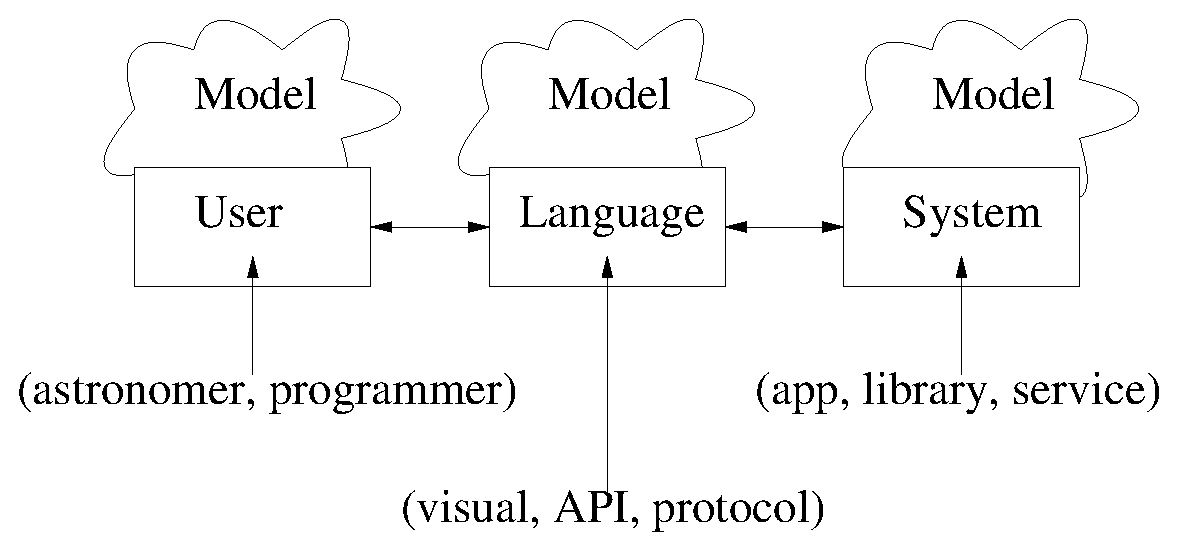
\includegraphics[width=\hsize]{models.eps}
\end{myslide}

\begin{myslide}{(Users)}
In this picture, the `users' include, but are not limited to, the
person handling the mouse.  Thus we might find
  \begin{itemize}
    \item an astronomer is a \emph{user} using a UI to interact with an
      application
    \item \dots the developer of which is a \emph{user} of an API to
      interact with a library
    \item \dots which is a \emph{user} of a protocol to interact
      with a local/remote service.
  \end{itemize}
So we're not just talking about GUI design, here.

There are \emph{multiple} user/language/system sets.

Each model must be comprehensible.  But we don't have to cover everything.

\end{myslide}

\begin{myslide}{Languages II}
\vbox to 0pt{\hbox to \hsize{\hss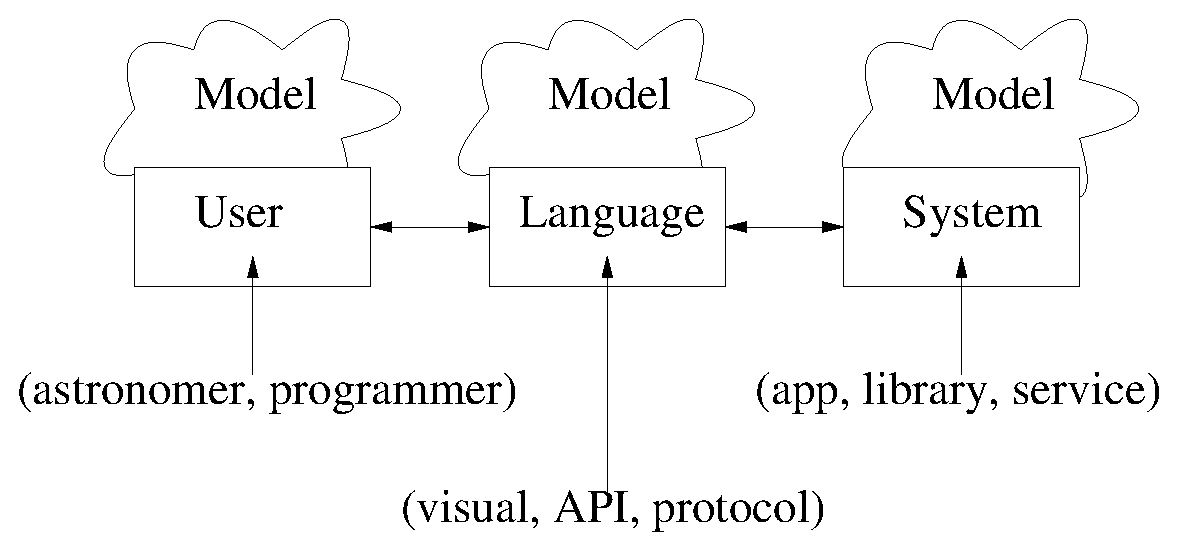
\includegraphics[width=0.5\hsize]{models.eps}}\vss}
\begin{itemize}
\item interface${}={}$`language'
\item \dots and thus a model
\item Systems are modelled
\item Users have/create models
\item \dots by reading documentation and using the language
\item If the three match, we get usable/correct/fast code
\item If not, not
\end{itemize}
Aren't mismatches inevitable?  What do a star and a database record
have in common except a tendency to generate entropy?
\end{myslide}

\begin{myslide}{Models are for thinking with}
A data model is the set of primitive concepts that we hope 
\begin{itemize}
\item \dots our user thinks with,
\item \dots the language expresses (in syntax),
\item \dots and the underlying system implements (in code)
\end{itemize}
If the model is made explicit at the beginning of the process, then we
can think with it, check it is consistent, both with itself and with
the outside world
%
%The DM is what will be implemented in code, not the syntax, so the
%language had better reflect it well to the user.
\end{myslide}

\begin{myslide}{So how do we make it explicit?}
\begin{itemize}

\item Obvious answers are XSchema, UML, Java class library

%\item But these come with a lot of extra baggage, which worms its way
%into the model: Do stars \emph{really} have methods?  Multiple
%containment/circular reference in XML

\item But extra baggage worms its way into the model: Do stars
  \emph{really} have methods?  Multiple containment/circular reference
  in XML
% Latter point is: eg, calibration image for more than one
% observation -- can express this in XML, but it's not necessarily
% natural. If you have `containement' relations, get them for free in XML.

\item So either decide that you \emph{want} the baggage, or use a
  more neutral modelling language
% which describes things at a more primitive level
\item RDF is another possibility, with little baggage
\end{itemize}
As long as you separate modelling from syntax (that is, the set of
rules for bytes/angle-brackets) you can \emph{discuss} the syntax --
if you don't you have to muddle the two together.
\end{myslide}

% 
% \section{Language, models and usability}
% 
% In linguistics, the well-known Sapir-Whorf hypothesis states that the
% way we conceive of the world depends on the language we use to
% describe it.  Or more compactly, we can only think what we can
% say.
% 
% This matters to us, since when we create software systems, we are
% often creating a `language' -- in a user-interface, an API or a
% protocol -- which users must employ to interact with an underlying
% system, be it an application, a library, or a remote service (here and
% below, we use the term `users' to apply both to astronomers using a
% mouse and programmers using an API or protocol).  If there is a good
% three-way match between the concepts in the user's head, the concepts
% implied by the language, and the concepts implicit in (some aspect of)
% the system's actual design, then the user's interactions with the
% system will be straightforward and largely error-free.  If there is a
% mismatch, they will not.  This is not just a matter of user-interface
% design; if the `user' is a programmer working with an API or a
% protocol, then this three-way match will help them write correct code
% faster, and produce an application which will in turn be usable by its
% eventual audience.
% 
% We can all think of systems which fail to exhibit this full match, but
% in some cases, surely a mismatch is inevitable.  After all, a star and
% a database record surely have nothing in common except a tendency to
% generate entropy.  This is why we need a data model.
% 
% A data model is the set of primitive concepts that we hope our user
% thinks with, the language expresses, and the underlying system
% implements; it is the rendezvous which helps the system as a whole
% hang together.  If the model is made explicit during the development
% process, then it can itself be examined, criticised, and checked for
% consistency with itself and with the external system it is
% supposed to model, whether that is, say, CDS or `a quantity'.  Once
% the model is itself part of the language of development, we can think
% with it, and talk about it, rather than merely mumble.
% 
% This immediately prompts the question of just how we make the model
% explicit.  There are several obvious answers to this, of which the
% most currently fashionable will be XSchema, UML, and `a Java
% class library'.  The problem with each of these is that they each come with
% far too much baggage.  This is another aspect of the Sapir-Whorf
% hypothesis: we tend to see the world in terms of the
% structure of the language we use to describe it.  That means that if
% we use XSchemas to model the world, we will discover that the world is
% made of things enclosing other things, with attributes, and if we use an O-O language,
% the world turns out to have methods.  That is, our choice of modelling
% language biases our model to have certain features, \emph{irrespective} of
% whether these features are present in the system being modelled.
% 
% A separate problem is to start thinking about syntactical or
% presentational details too early.  If we retrofit a data model, it
% will end up being a poor model of the world, but an excellent
% model of our syntax.
% % During the UCD modelling effort, we found ourselves asking questions
% % which purported to be about astronomy, but which were really about
% % underscores.
% 
% There are two strategies to deal with this.  The first is to embrace
% the problem, acknowledge that our choice of language is not neutral,
% and make sure that choice is a good one.  The second is to choose a
% more primitive modelling language, which will push fewer things into
% the model.  We will return to this question in section~\ref{s:techniques}.


\end{slidegroup}


\begin{slidegroup}{votable}{VOTable and other models}

\begin{myslide}{VO data models}
  There are already several data models in the air
  \begin{itemize}
    \item VOTable -- resources within resources within\dots
    \item SIAP -- `get me a picture like\dots'
    \item UCD and Quantities -- what \emph{is} an Observation anyway?
    \item WCS -- `where did that image come from?'
  \end{itemize}
Note that several of these use VOTable: make sure to distinguish
VOTable(model) from VOTable(syntax).
% How do we serve lazy/rushed/generic developers?
% Cut down VOTable?
% Work out what their DM is and \emph{then} write it down.
\end{myslide}

\begin{myslide}{VOTable is good}
Viewed as a way of\dots
\begin{itemize}
\item \dots archiving catalogue metadata,
\item \dots transporting catalogues from catalogue producers to catalogue
consumers,
\item \dots encoding \emph{all} available information about a
catalogue or image
\end{itemize}
\dots VOTable is excellent.  There's a good match here between system,
language and user.

VOTable is expressive, recursive, and flexible.  \emph{But\dots}. 
\end{myslide}

\begin{myslide}{VOTable is hard}

\dots it's expressive, recursive, and flexible.
\begin{itemize}
  \item These are \emph{good} things if you're an archivist.  But
    \emph{bad} things if all you want is an image
  
  \item The problem is not with VOTable; instead there's \emph{more than one
model}, because there's more than one constituency of users.
How do we serve busy/ignorant/generic developers?
\end{itemize}
  
\end{myslide}

%% \begin{myslide}{VOTable is hard}
%% \dots it's expressive, recursive, and flexible.

%% These are \emph{good} things if you're an archivist.  But \emph{bad}
%% things if all you want is an image.  So:
%% \begin{itemize}
%% \item extend VOTable?  \emph{No!}: that would just make it more complicated
%% \item simplify VOTable -- miniVOTable?  Probably not: might not
%%   really address the problem
%% % that limits the flexibility without necessarily addressing the problem
%% \item provide libraries?  Possibly\dots
%% \end{itemize}
%% The problem is not with VOTable; instead there's \emph{more than one
%% model}, because there's more than one constituency of users.
%% How do we serve lazy/igorant/generic developers?
%% % (ie, programmers professional and casual).
%% \end{myslide}

\begin{myslide}{VOTable and data consumers}
\vbox to 0pt{\hbox to \hsize{\hss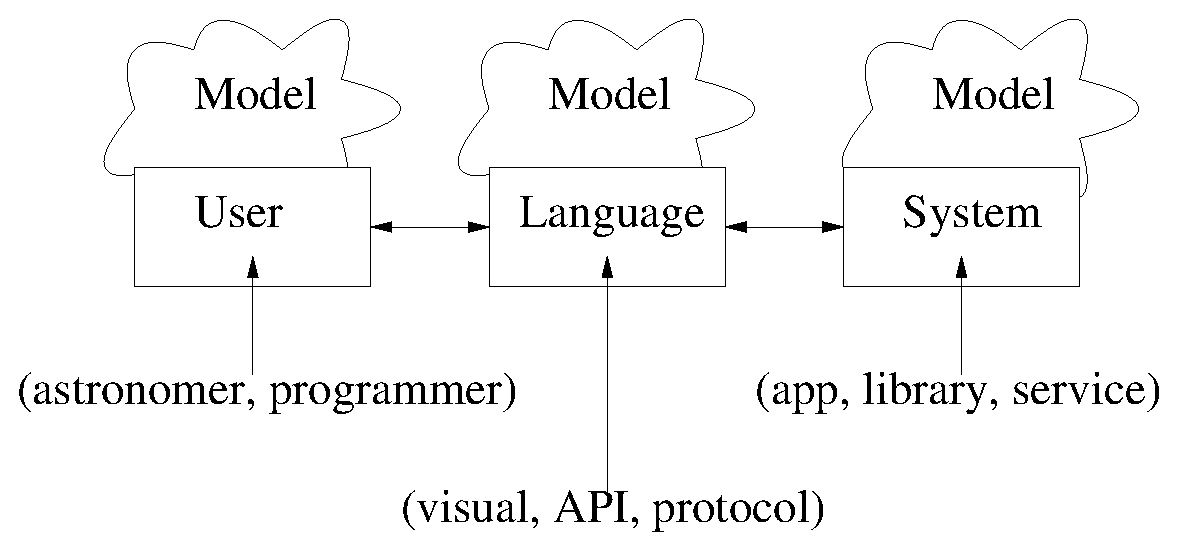
\includegraphics[width=0.5\hsize]{models.eps}}\vss}
\begin{itemize}
\item \begin{minipage}{0.5\hsize}
      \raggedright
      Data consumers (query agent, programmer) have a simple-minded model.
      \end{minipage}
\item \begin{minipage}{0.5\hsize}
      \raggedright
      Because there's multiple models, we
      don't have the three-way match any more; so lower software
      quality.
      \end{minipage}
\item Step 1: identify and express the data consumer's model
\item Step 2: \emph{then} work out how to map one model to the other
in principle, at the system end
\item Step 3: \emph{then} choose syntax/technology
\end{itemize}
\end{myslide}

\begin{myslide}{What to do?}
  
\begin{itemize}
\item extend VOTable?  \emph{No!}: that would just make it more complicated

\item simplify VOTable -- miniVOTable?  Maybe -- might not
  really address the problem

\item provide libraries/alternative syntax?  Possibly\dots
\end{itemize}

\end{myslide}

\begin{myslide}{UCDs}
  \begin{verbatim}
    _x rdf:type :pos.eq.ra .
    _x :stat.err "0.5arcsec" .
  \end{verbatim}
\begin{itemize}
\item Thus \texttt{pos.eq.ra} appears to be a type/class,
  \texttt{stat.err} is a property
\item Did we want that?
% Did we know that?  Did we mean that?  Do we want that?
\item Is this what we want \texttt{stat.err, pos.eq.ra} to mean?
\item If not, what?
\item Could we turn this into syntax $x$ if we wanted?  And
if not, isn't it lucky we didn't start with that syntax?!
\item Are there things the proposed syntax can't express?
%\item  Are there
%things we could think with the modelling language that we'd want to
%communicate but couldn't with the proposed syntax?

% At this point we can think about serialising this in syntax,
% confident that we are clear about the meaning.  We can have that
% confidence because we gave ourselves the words to think about it with.
\end{itemize}

\end{myslide}

\end{slidegroup}

% We contend that there is in fact more than one model relevant to the
% VO, and that while the VOTable model is an excellent and valuable fit
% to the archivists' model of data, it may be a poor match for many
% users or (which is much the same thing) for the software written to
% service the sort of end-user astronomical applications which the VO
% targets.



\begin{slidegroup}{tech}{Modelling technologies}

% Modelling work in other areas shows the importance of abstraction in
% the concrete goal of freeing software design from the particulars of
% any single implementation. This is extremely important for the VO
% because it allows us, and the software we write, to deal with the
% essentials of the data rather than the superficial aspects of a
% particular format such as XML or FITS. We discuss the work that we and
% others have been doing within this context; with this in mind, we will
% also review some of the various modelling languages available, such as
% XSchemas, UML, OMG MDA, HUTN, RDF, and Topic Maps.
% \end{abstract}

\begin{myslide}{XSchema}
\begin{itemize}
\item Well-known: XML instance syntax
\item Verbose
\item Complicated: the main benefit is \dots
\item Elaborate type system, looks familiar to database people; also this
is the type system used by other W3C standards
\item Langauges like RelaxNG have easier-to-read syntax and can
translate back-and-forth to XSchema
\item Not really a modelling language, but modelling is involved in
writing a schema
\end{itemize}
\end{myslide}

\begin{myslide}{UML}
\begin{itemize}
\item For designing object-oriented libraries
\item So it's usable for general modelling, to the extent that an object
  model is appropriate for you
%\item Emphasises processing and interfacing over data

\item O-O notions of subclassing and object manipulation are natural
  in UML, in the way that containment is natural in XML

\end{itemize}
\end{myslide}

\begin{myslide}{Object modelling languages}
If you've decided that an object model is for you, then
acronym salad: UML, IDL, CORBA,
Java/EJB/.NET/SOAP.

OMG standards to generate UML/XML
models from `metamodels', then generate the code to tie them together.
\begin{itemize}
% HUTN <http://www.dstc.edu.au/Research/Projects/Pegamento/hutn/>
% OMG MDA at <http://www.omg.org/mda/>
% OMG XMI at <http://www.omg.org/technology/documents/formal/xmi.htm>
\item MDA (Model Driven Architecture): platform-independent
  application descriptions
\item XMI (XML Metadata Interchange): XML-based modelling language
intended to help generate and exchange mutually consistent XSchemas,
UML and code (CORBA and IDL interfaces).
\item HUTN (Human-Usable Textual Notations): how to write XMI without
angle-brackets.
\end{itemize}
Buzzzzzzzz.
\end{myslide}

\begin{myslide}{RDF and OWL}
\begin{itemize}
\item W3C standard
\item RDF is a set of primitive ideas for representing relations between
entities -- subject-predicate-object
\item Base RDF is mostly concerned with syntax
\item RDFSchema and OWL (Ontology Language for the Web) supplements RDF with
properties such as \texttt{minCardinality}, \texttt{equivalentClass}
and \texttt{intersectionOf} which support basic reasoning
\item Notation3 is \emph{much} more readable than ugly RDF/XML: for example
\texttt{\#apple :obs.mass "200g" .}
\end{itemize}
\url{http://www.astro.gla.ac.uk/users/norman/note/2003/rdf-intro/}
\end{myslide}

\end{slidegroup}

\begin{myslide}{So\dots}
  \begin{itemize}
    \item The VO will have multiple user/language/system sets
    \item \textbf{Each \emph{potentially} has a separate model, and
      this should be acknowledged and planned for}
    \item Three-way consistency and intelligibility are more important
      than having one model for the whole VO
    \item Linking these independent models might be more profitable
      than attempting to develop some Grand Unified Model
    \item \textbf{Making your DM explicit lets you think about it --
      syntax comes \emph{second}}
    %\item Modelling is separate from syntax
    \item If we think about syntax too early, we end up modelling the syntax
  \end{itemize}
\end{myslide}


\end{document}
